\subsection{Numerical Results}\label{sec:numResultX}

We concentrate our experiments on Brownian trajectories.  
First, we illustrate %visualize and compare 
the  path  approximations seen earlier (Karhuhen-Loève, L\'evy-Cieselski, Signature).
Figure \ref{fig:projPath} displays the projections using $K=8$ basis elements. We naturally notice similarities between the Karhunen-Loève transform and the L\'evy-Cieselski construction with Fourier cosines, both 
obtained by superposing trigonometric functions.

Let us gauge the accuracy of the above approximations for Brownian trajectories, in terms of (i) 
    $\epsilon^{K,\frakF}$ and (ii) variance explained 
    $ \vartheta^{K,\frakF} := \frac{\lVert X^{K,\frakF}  \rVert^2_{*}}{\left \lVert X \right \rVert^2_{*}}.$ 
To compute (i), (ii) and the coefficients $(X,F_k)_{\calH}$, we discretize the interval $[0,1]$ a regular partition made of $N = 10^4$ subintervals. 
\Cref{fig:Error_VarExp} displays the evolution of $\epsilon^{K,\frakF}$, $\vartheta^{K,\frakF}$ for $K\in \{1,\ldots,128\}$. The Karhunen-Lo\`eve expansion clearly dominates the other projections, although being asymptotically equivalent to the L\'evy-Cieselski construction with Fourier cosine basis. Besides, the $L^2(\mathbb{Q} \, \otimes \, dt)$ convergence of the Brownian bridge construction (L\'evy-Cieselski with Haar basis) is non-monotonic. Indeed, a bump appears until a full cycle of the dyadic partition is completed. 
Lastly, the slopes in the log-log convergence plot  (left chart of \Cref{fig:Error_VarExp}) 
are roughly equal to $-1$. Put differently,  the squared approximation error is of order $\calO(\frac{1}{K})$, confirming our findings from the  above examples.

\begin{figure}[t]
    \centering
    \caption{$L^2(\mathbb{Q} \, \otimes \, dt)$ error and variance explained.}
    \vspace{-2mm}
    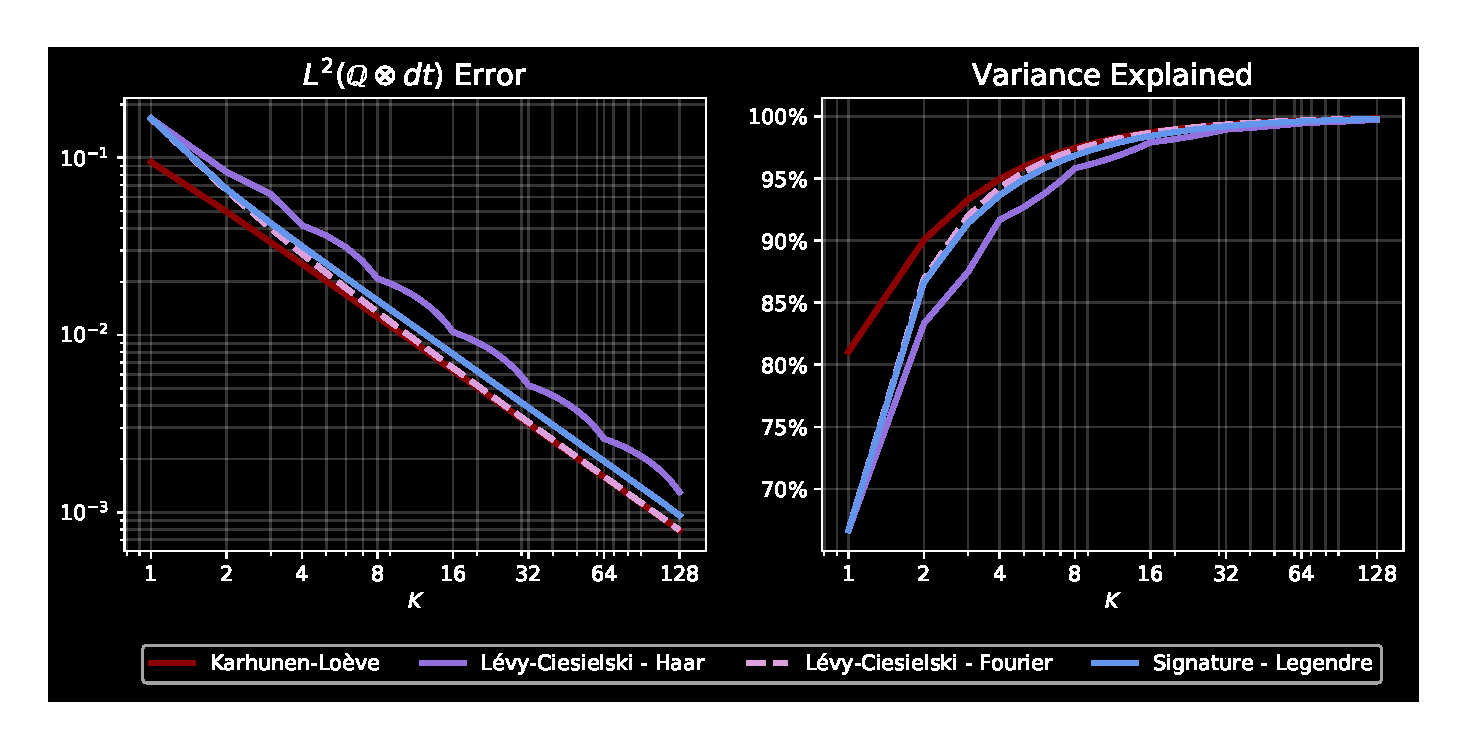
\includegraphics[scale = 0.45]{KL/Figures/Err_VarExp.pdf}
    \label{fig:Error_VarExp}
\end{figure}